% Compact PGFPlots panel for sampled two_gross288 BSC correction-class derivative.
% Requires \usepackage{pgfplots} and \pgfplotsset{compat=1.18}.
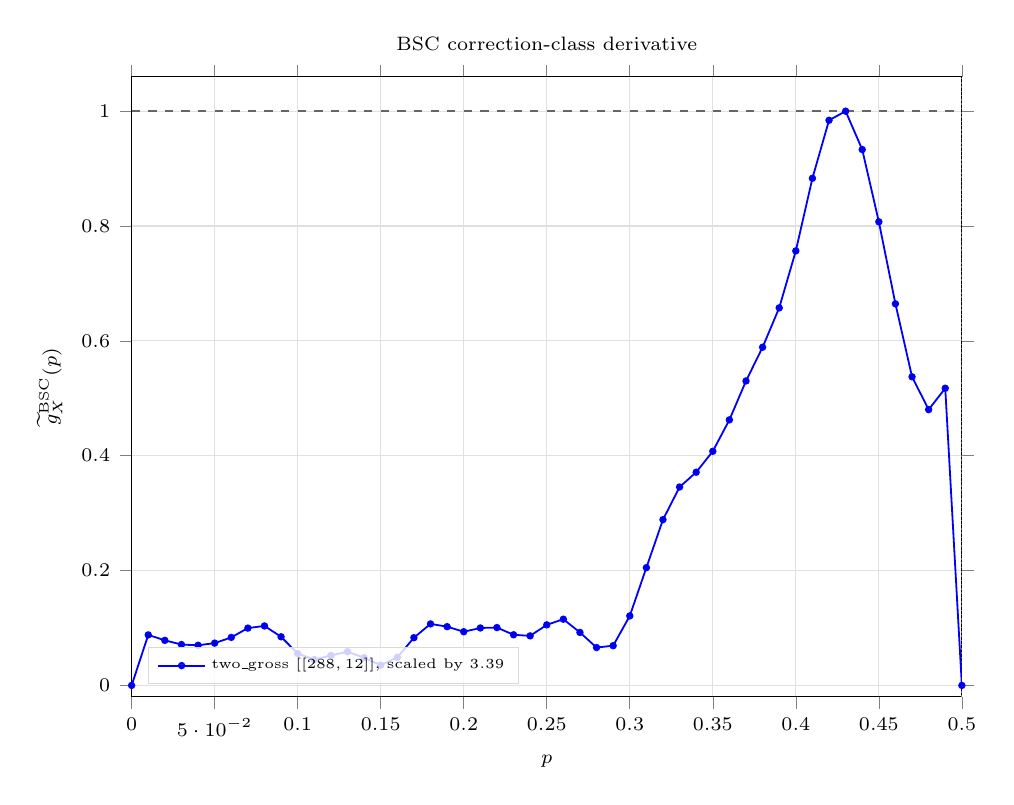
\begin{tikzpicture}
\begin{axis}[
  name=scaledBSCGEXITTwoGross288Axis,
  width=\linewidth,
  height=0.78\linewidth,
  title={BSC correction-class derivative},
  title style={font=\scriptsize},
  xlabel={$p$},
  ylabel={$\widetilde g_X^{\rm BSC}(p)$},
  xmin=0, xmax=0.5,
  ymin=-0.02, ymax=1.06,
  grid=both,
  major grid style={black!12},
  minor grid style={black!6},
  tick align=outside,
  tick label style={font=\scriptsize},
  label style={font=\scriptsize},
  legend cell align={left},
  legend style={draw=black!15, fill=white, fill opacity=0.82, text opacity=1, at={(0.02,0.02)}, anchor=south west, font=\tiny},
]
\addplot[black!60, densely dotted, line width=0.55pt, forget plot] coordinates {(0.5,-0.02) (0.5,1.06)};
\addplot[black!60, dashed, line width=0.55pt, forget plot] coordinates {(0,1) (0.5,1)};
\addplot+[color=blue, mark=*, mark size=1.0pt, line width=0.65pt]
coordinates {(0,0) (0.01,0.087990167404) (0.02,0.0784667417244) (0.03,0.0711813369313) (0.04,0.0698847741102) (0.05,0.0736582906386) (0.06,0.0836141178034) (0.07,0.0998114362745) (0.08,0.10358934328) (0.09,0.0846924304739) (0.1,0.0555401093216) (0.11,0.0449811850564) (0.12,0.0522371839167) (0.13,0.0587147090151) (0.14,0.0482056508983) (0.15,0.0352464754446) (0.16,0.0488452856257) (0.17,0.0830800731212) (0.18,0.107123112634) (0.19,0.102338019367) (0.2,0.0935030553789) (0.21,0.10004325068) (0.22,0.100770626247) (0.23,0.0882097225179) (0.24,0.0862804177668) (0.25,0.105466616487) (0.26,0.115292906935) (0.27,0.0922598106418) (0.28,0.0659439578044) (0.29,0.0692099973794) (0.3,0.121012125583) (0.31,0.205073609391) (0.32,0.28867892656) (0.33,0.345504812611) (0.34,0.371254610333) (0.35,0.407759646912) (0.36,0.462447848155) (0.37,0.530194739289) (0.38,0.588968129025) (0.39,0.657521099316) (0.4,0.756705407485) (0.41,0.88315174706) (0.42,0.984138921055) (0.43,1) (0.44,0.933148138313) (0.45,0.807412771816) (0.46,0.664541666158) (0.47,0.537449725163) (0.48,0.48032194755) (0.49,0.517490580227) (0.5,0)};
\addlegendentry{two\_gross $[[288,12]]$, scaled by $3.39$}
\end{axis}
\end{tikzpicture}
